\subsection{Resultados da busca de revis\~ao}\label{subesec:resul da revisão}


Nesta seção serão apresentados os resultados da pesquisa utilizando algum software, a fim de estipular o melhor uso de cada banco de dados utilizado durante o trabalho. Assim, pode-se começar com a análise no \textit{software VOSviewer}. 

\begin{figure}[htp!]
	\centering
	\caption{Palavras-chave mais populares na Scopus.}
	\label{fig:scopus-09-08}
	\includegraphics[width=0.9\linewidth]{Revisao/Figuras/"scopus 09-08"}
	
	\vspace{0.2cm}
	Fonte: Elaboração própria a partir de dados da Scopus (2016 a 2022)
\end{figure}
Na figura \ref{fig:scopus-09-08} há uma lista das palavras mais usadas como sinônimos da palavra \textit{time series analysis} ou juntas no corpo do texto dos artigos.
A análise da base de dados no scopus foi feita na ferramenta que mostra as palavras-chave que podem ser relacionadas em cada campo de busca, com isto tem uma visão ampla do que pode ter correlação com as palavras-chave mãe da busca.

Na relação entre as palavras-chave neste primeiro momento, foi obtido um resultado de 3484 palavras-chave, 212 atingindo o limite, lembrando que as palavras base a partir das quais se deve chegar ao texto \textit{``time series forecasting and time series analysis''} em Scopus.



\begin{figure}[htpb!]
	\centering
	\caption{Palavras-chave mais populares na Web of Science}
	\label{fig:web-09-08}
	\includegraphics[width=0.8\linewidth]{Revisao/Figuras/"web 09-08"}
	
	
	
	\fonte{Elaboração própria a partir de dados da Web of Science (2016 a 2022)}
\end{figure}


Na Figura \ref{fig:web-09-08} a análise do banco de dados Web of Science foi feita na ferramenta que mostra as palavras-chave que estão relacionadas em cada campo de busca, com isto você pode ter uma visão ampla do que tem correlação com as palavras-chave mãe da busca.

Na relação entre as palavras-chave neste primeiro momento, teve um resultado de 305 palavras-chave, 13 atingem o limite, lembrando que as palavras base para o resultado foi \textit{``time series forecasting and time series analysis''} na web of science.

O único banco de dados que não será mostrado aqui é o banco de dados Lente, porque é um excelente banco de dados e ainda não retornou muito na busca que foi feita. O site do lens retornou apenas 11 artigos com os filtros aplicados. Na \ref{etp:rev-1} é observado o campo de busca que foi usado nesta busca que deu apenas 11 artigos.



\begin{table}[htpb!]
	\caption{Cruzamento de palavras-chave através da aplicação de filtros de ano e de linguagem}\label{tb1}
	\centering
	\begin{tabular}{@{}cp{2cm}p{1cm}p{2cm}p{1cm}p{2cm}p{2cm}p{2cm}@{}}
		\toprule
		Bases                             & \multicolumn{5}{c}{Palavras Chaves}                                                         & Resultado \\ \midrule
		\multirow{2}{*}{Scopus}           & time   series forecasting & AND & time   series analysis    &     &                         & 490       \\
		& nonlinear forecasting     & AND & time   series forecasting &     &                         & 8         \\
		\multirow{2}{*}{Web   of Science} & time   series forecasting & AND & time   series analysis    &     &                         & 126       \\
		& nonlinear forecasting     & AND & time   series forecasting &     &                         & 14        \\
		Lens                              & time   series forecasting & AND & time   series analysis    & AND & nonlinear   forecasting & 11        \\
		\multicolumn{6}{c}{Total}                                                                                                       & 649       \\ \bottomrule
	\end{tabular}
	
	\fonte{Elaboração própria a partir de dados da Scopus, Lens e Web of Science (2016 a 2022)}
\end{table}


Na Tabela \ref{tb1}, ela lista as palavras-chave para cada base e aumenta a quantidade de artigo em todas as bases, mas esta tabela está com os dados brutos que não foram eliminados as duplicatas, portanto, usando o \textit{software mendeley} para remover as duplicatas devolve apenas 308 artigos.




\begin{figure}[htp!]
	\centering
	\caption{Analise das quantidades de artigos em relação aos anos.}
	\label{fig:regressao-linear-dos-artigos-baseados-nos-anos}
	\includegraphics[width=0.9\linewidth]{Revisao/Figuras/"regressão linear dos artigos baseados nos anos"}
	
	\fonte{Elaboração própria a partir de dados da SANEPAR (2018 a 2020)}
\end{figure}

A figura \ref{fig:regressao-linear-dos-artigos-baseados-nos-anos} tem com abcissas e ordenadas anos e artigos, assim a relação entre a data de publicação dos artigos ao longo do tempo.

Um número considerável de artigos para analisar na Figura \ref{fig:regressao-linear-dos-artigos-baseados-nos-anos} uma análise foi feita com base em uma regressão linear dos artigos ao longo dos anos de 2016 a 2022, nesta análise obteve a seguinte equação de regressão linear:


\begin{eqnarray}
	y(x)&=&8,3571x - 16803 \qquad \text{Com } R^2=0,3062\label{eq1}
\end{eqnarray}

Com $y(x)$ a equação da reta na equação \eqref{eq1}. $8,3571$ é o coeficiente angular do gráfico de $ y(x)$, $16,803$ é o coeficiente linear, ou o ponto de intersecção com o eixo $y$, $x$ é a variável independente.

Este coeficiente indica a proporção da variância da variável dependente que pode ser atribuída estatisticamente ao conhecimento de uma ou mais variáveis independentes \citeonline{coeficiente}. 

O coeficiente de determinação mede a relação que existe entre a variável dependente e as variáveis independentes, indicando que porcentagem da variação explicada pela regressão representa da variação total. Quando:

$R^2=1$: todos os pontos observados estão exatamente na reta de regressão (ajuste perfeito), ou seja, as variações de $y$ são de $100\%$ explicadas pela variação de $x_n$ através da função especificada, sem desvios em torno da função estimada. 

$R^2=0$: conclui-se que as variações de $y$ são exclusivamente aleatórias e a introdução das variáveis $x_n$ no modelo não incorporará nenhuma informação sobre as variações de $y$.

\begin{equation}
	R^{2}=\frac{\left(\sum X . Y-\frac{\sum X \cdot \sum Y}{n}\right)^{2}}{\left[\sum X^{2}-\frac{\left(\sum X\right)^{2}}{n}\right] \cdot\left[\sum Y^{2}-\frac{\left(\sum Y\right)^{2}}{n}\right]}=(r)^{2}\label{eq2}
\end{equation}

Na equação \eqref{eq2} $X,Y$ é dado pelas coordenadas no plano cartesiano como por exemplo o par encomendado $(x,y)$. 
Na equação \eqref{eq1} observa-se que obteve o $R^2=30\%$ isto implica que a linha de regressão será influenciada pelo $R^2$ que foi encontrado.

Embora seja uma análise muito simples que foi realizada com a relação entre número de artigos e anos, ainda é uma validação muito boa para olhar para o teste F de significância que é dado o significado tem que ser sempre $F<5\%$ este teste também é chamado de p-valor.

Tendo estes valores, é possível analisar o significado extremo da linha de regressão e observar que 2021 foi o ano em que a maioria dos artigos foram publicados sobre este tema da séries temporais.

\begin{table}[H]
	\centering
	\caption{Fator de impacto}\label{tb2}
	\begin{tabular}{@{}cp{3cm}p{3cm}c@{}}
		\toprule
		Revista cientíica      & Quantidade de plubicação & Qualidade da revista & H-INDEX \\\midrule
		Neurocomputing         & 27                         & Q1                     & 143     \\
		IEEE Access            & 18                         & Q1                     & 127     \\
		Applied Soft Computing & 12                         & Q1                     & 143     \\
		Energies               & 11                         & Q2                     & 93      \\
		Energy                 & 11                         & Q1                     & 343     \\ \bottomrule
	\end{tabular}
	
	
	\fonte{Elaboração própria a partir de dados da Scopus, Lens e Web of Science (2016 a 2022)}
\end{table}

Na Tabela \ref{tb2} mostra revistas que a maioria publica artigos sobre este assunto, já que muitas revistas não estão localizadas no Brasil e têm seus nomes em inglês, mas todas as revistas com um fator de impacto muito alto como \textbf{A1} têm uma correlação com as áreas de \textbf{informática, engenharia e matemática}.

\begin{figure}[htpb!]
	\centering
	\caption{Relação de autores entre artigos publicados}
	\label{fig:autores-relacao-entre-artigos-publicados}
	\includegraphics[width=0.8\linewidth]{Revisao/Figuras/"Autores Relação entre artigos publicados"}
	
	
	\fonte{Elaboração própria a partir de dados da Scopus (2016 a 2022)}
\end{figure}

\begin{figure}[htpb!]
	\centering
	\caption{Ligação bibliográfica entre os autores}
	\label{fig:autores}
	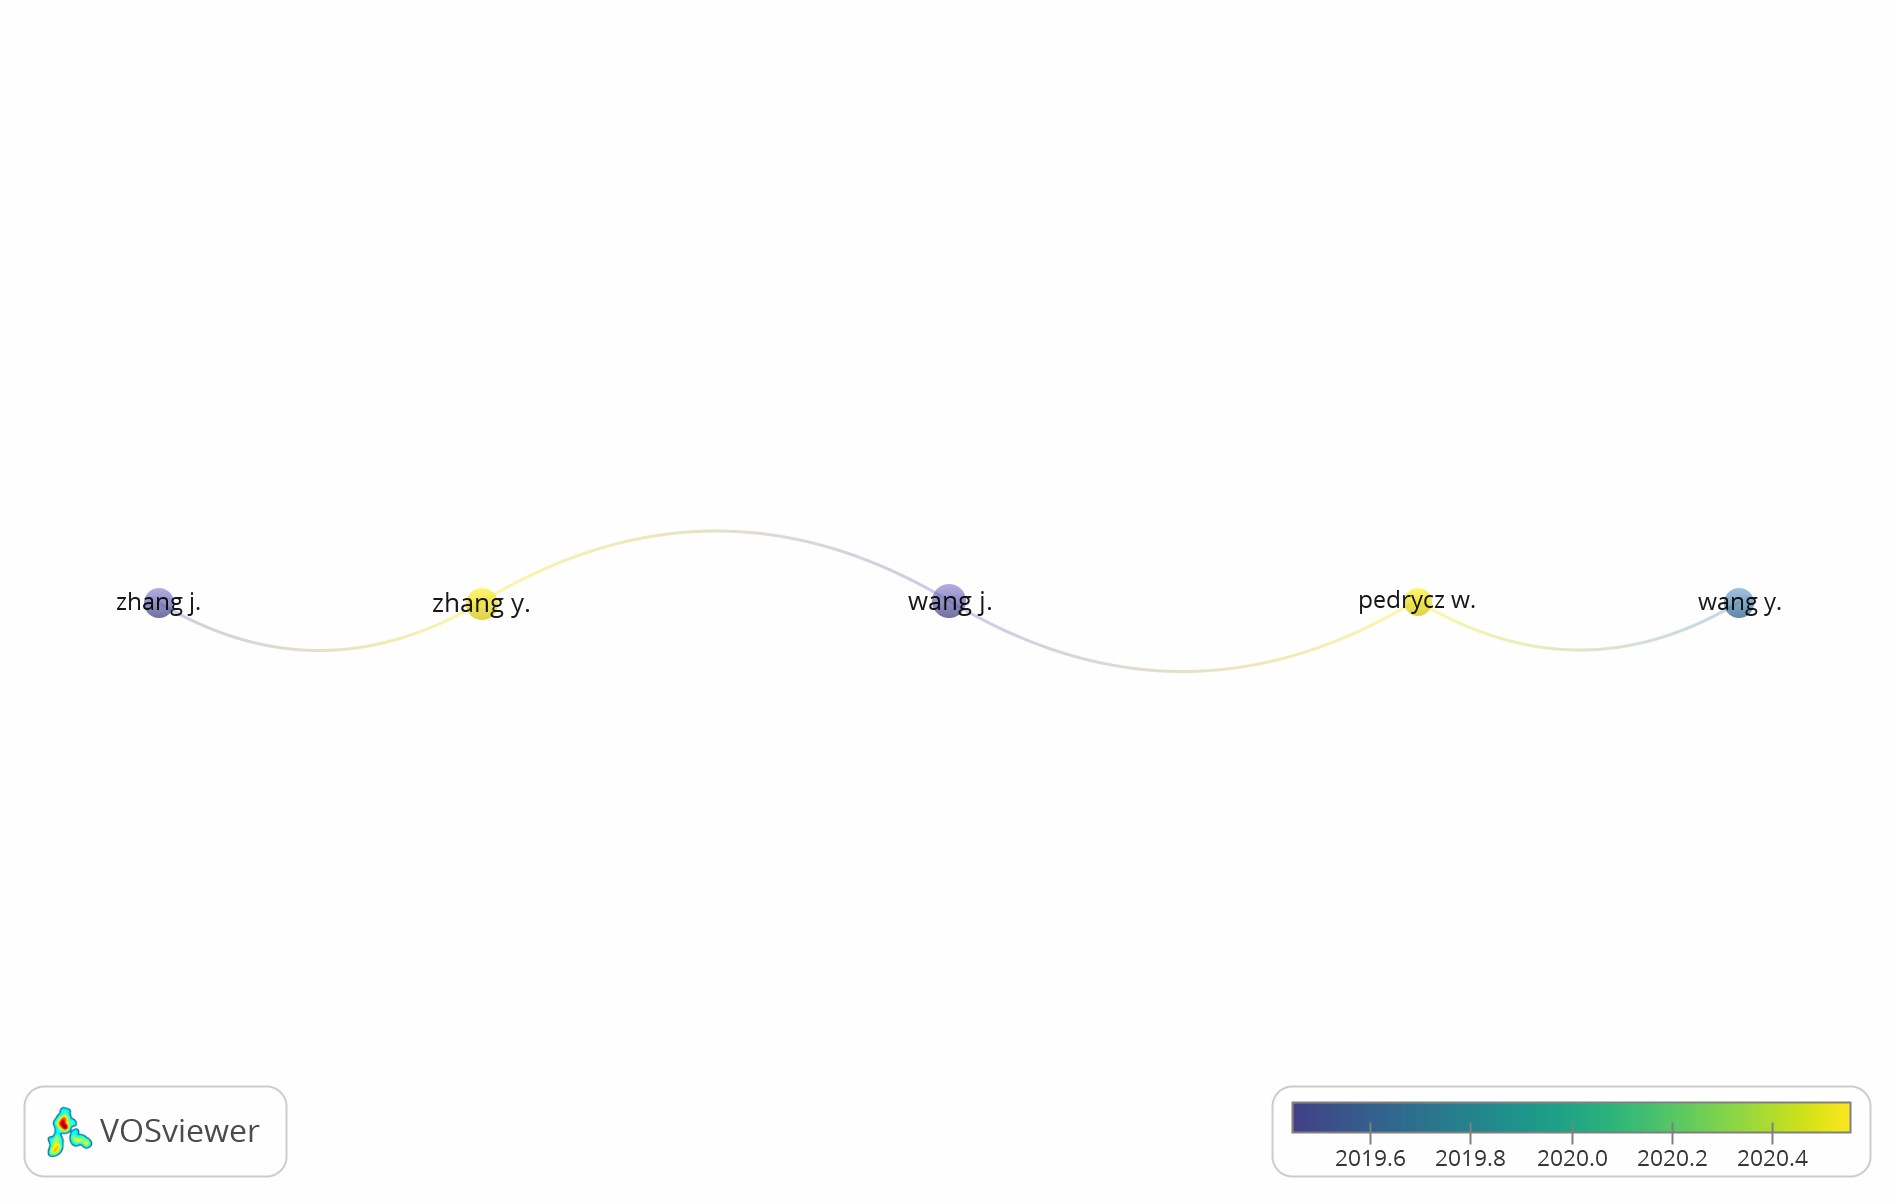
\includegraphics[width=0.8\linewidth]{Revisao/Figuras/Autores}
	
	\fonte{Elaboração própria a partir de dados da Scopus (2016 a 2022)}
\end{figure}

Respondendo a um problema aqui colocado, o \ref{questão:rev1} usa a Figura \ref{fig:autores-relacao-entre-artigos-publicados} com um gráfico de histograma para ser mais visível que os autores que mais publicaram neste tópico no gráfico colocam os autores que tiveram publicação maior que 4 e com isto não coloca todos os autores considerando os autores que publicaram mais de 4 artigos neste tópico de 2016 a 2022.


\begin{figure}[htpb!]
	\centering
	\caption{Mapa mundial da publicação de artigos em todo o mundo}
	\label{fig:mapa-mundi-artigos}
	\includegraphics[width=1\linewidth]{Revisao/Figuras/"mapa mundi artigos"}
	\vspace{0.2cm}
	
	\fonte{Elaboração própria a partir de dados da Scopus, Lens e Web of Sicence (2016 a 2022)}
\end{figure}

Na pergunta de pesquisa \ref{questão:rev2} é respondido com a Figura \ref{fig:mapa-mundi-artigos} os países que mais público sobre o assunto em escala desde a maior publicação até a menor em escala, como segue China - 119, Estados Unidos - 67, Índia - 57, Brasil - 32, Espanha - 28, Reino Unido - 25, Austrália - 24, Irã - 18, Malásia - 17, Canadá - 16. O mapa não mostra todos os países com seus números de publicação.


\begin{figure}[htpb!]
	\centering
	\caption{Áreas de aplicação do tema}
	\label{fig:areas}
	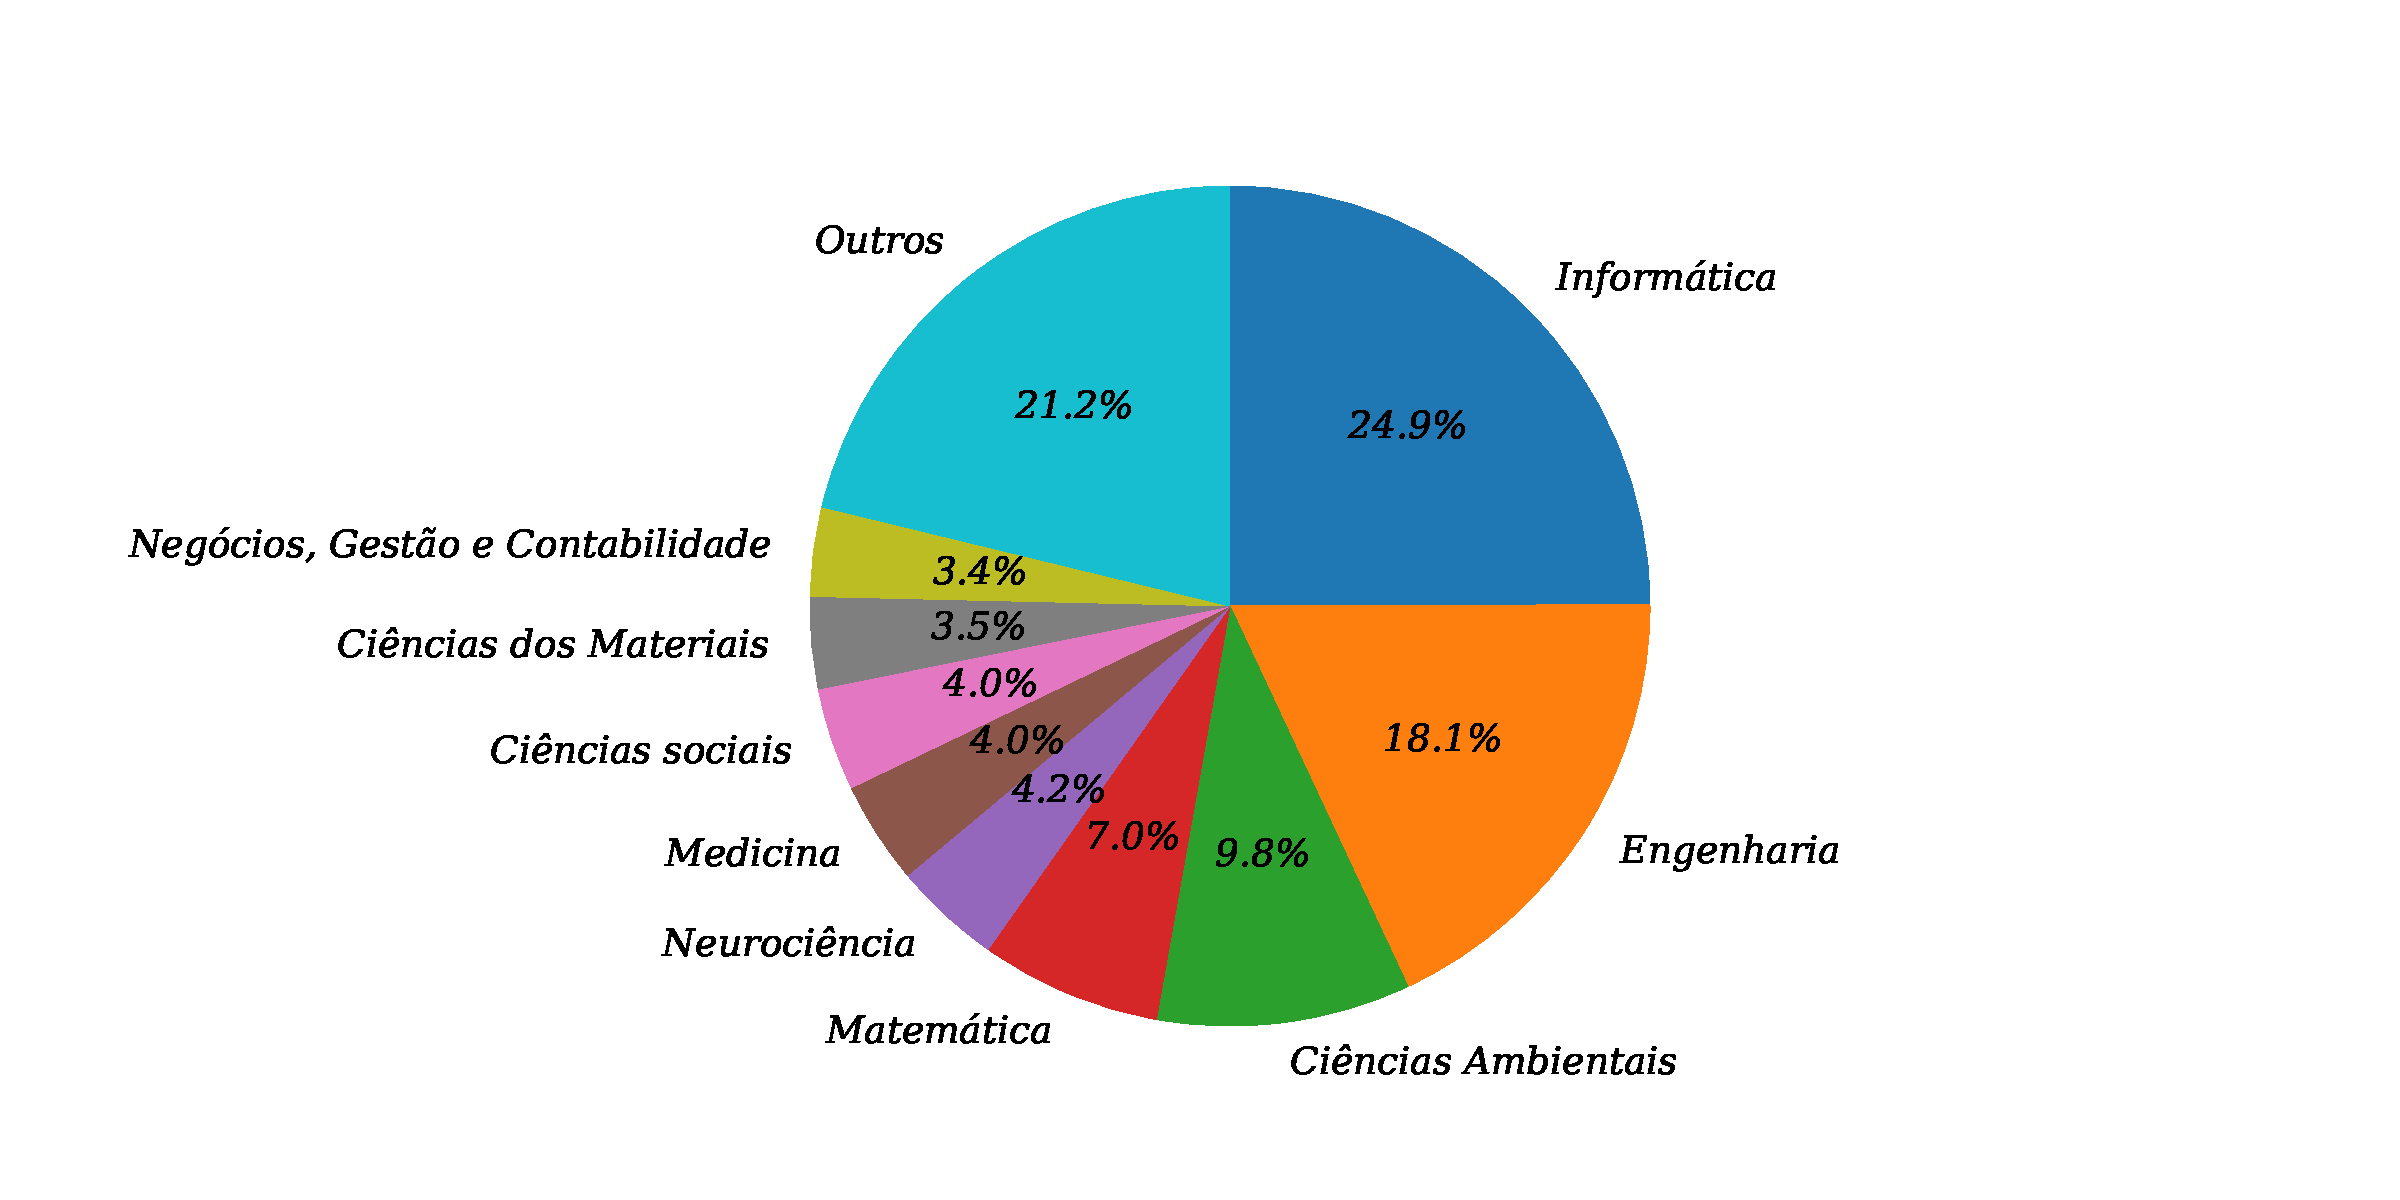
\includegraphics[width=0.9\linewidth]{Revisao/Figuras/areas}
	\vspace{0.2cm}
	
	\fonte{Elaboração própria a partir de dados da Scopus, Lens e Web of Sicence (2016 a 2022)}
\end{figure}


Pergunta de pesquisa \ref{questão:rev3} para responder a esta pergunta, foi feito um gráfico circular para rotular as áreas que têm mais publicação no tempo escolhido na revisão. A Tabela \ref{tb3} mostra os valores de cada área e sua quantidade de publicação. 

\begin{table}[!htb]
	\centering
	\caption{Áreas e seus valores respetivos de artigos em cada área.}\label{tb3}
	\begin{tabular}{@{}ll@{}}
		\toprule
		Informática                      & 240 \\ \midrule
		Engenharia                       & 174 \\
		Ciências Ambientais              & 94  \\
		Matemática                       & 67  \\
		Neurociência                     & 40  \\
		Medicina                         & 38  \\
		Ciências sociais                 & 38  \\
		Ciências dos Materias            & 34  \\
		Negócios, Gestão e Contabilidade & 33  \\
		Outros                           & 204 \\ \bottomrule
	\end{tabular}

	
	\fonte{Elaboração própria a partir de dados da Scopus, len e Web of Sicence (2016 a 2022)}
\end{table}


Na última pergunta de pesquisa \ref{questão:rev4} foi feita uma pesquisa sobre alguns dos artigos mais influentes na revisão, esses artigos retratam alguns métodos sobre séries temporais dos artigos dos autores \citeonline{Golyandina2020, Kumar2021, Xie2019, Lara-Benitez2021, Ahmad2018, CarvalhoJr.2019, Tan2021, Liu2019, Liu2021, Rossi2018, Soyer, Martinovic2020a, Ursu2016, Wang2016, Shih2019a, Moon2019, Chou2018, Bergmeir2018, Boroojeni2017, Chou2018a, Coelho2017, Du2020, Sadaei2019, Salgotra2020, Tyralis2017, Vlachas2020, Yang2019a, Shen2020, Sezer2020, Chen2018, Buyuksahin2019, Li2020, Kulshreshtha2020, Samanta2020, Xu2019, Graff2017, Taieb2016}
alguns métodos usados pelos autores para previsão de séries temporais e alguns modelos de análise da mesma previsão não-linear. 


\citeonline{Xu2019} no modelo híbrido, o modelo linear AR e LR ou o modelo ARIMA e o modelo DBN não-linear são explorados para capturar os comportamentos lineares e não-lineares de uma série temporal, respectivamente. \citeonline{Li2020} o desempenho de previsão da abordagem MAELS é comparado com os predecessores baseados na aprendizagem de máquinas de última geração como CNN, RNN, LSTM, ARIMA, e SVM-VAR. As abordagens, CNN, RNN e LSTM permitem o manuseio multivariado de entrada e saída, ARIMA usa dados passados para prever o futuro usando duas características principais: autocorrelação e médias móveis.


Assim, com esta revisão sistemática e análise de conteúdo, a resposta à pergunta de pesquisa feita no início do capítulo foi obtida.

Fora destes modelos, também há a atualização ARIMA que será utilizada nesta dissertação, pois SARIMA, SARIMAX ambos os modelos serão comparados para se obter o melhor modelo entre eles, fora disto também será utilizado o Light GBM e o XGBoost. Para as métricas de erro nesta dissertação serão utilizadas as seguintes métricas e explicadas no capítulo \ref{sec:base} MAE, MAPE e RMSE na literatura é um dos mais utilizados entre vários com, por exemplo, os $R^2$ citados \eqref{eq2} para as previsões futuras sempre foram confrontados com estas métricas de erro. os $R^2$ não são tão utilizados para comparação.